\section{Network architecture}\label{sec:network}
\Todo[inline]{Mention root joint}
\begin{itemize}
	\item basic principle of gans
	\item Basic architecture used in the paper
	\item Motivation for predicting depth offsets
	\item Mention batch norm not working with reference to other paper and communication with authors
	\item Projection and reprojection.
	\item Norm limb normalization
	\item Heuristic: If a random projection of a 3D pose is realistic, the 3D pose is also realistic
	\item mention residuals: $dx$ and $dy$ at normalization
\end{itemize}

\subsection{Generative Adversarial Networks}
Generative Adversarial Networks (GANs) have first been presented by \citet{goodfellow14} in 2014.
As the name suggests, they are generative models involving two adversary agents, a \emph{generator} and a \emph{discriminator}.
The discriminator $D$ tries to guess whether its input belongs to the real data distribution $p_{real}$ (the distribution to be learned) or to the distribution $p_{fake}$, which is implicitly captured by the generator.
The generator $G$ on his behalf tries to learn the distribution $p_{fake}$ such that it resembles $p_{real}$, and thus fool the discriminator into thinking that the data produced by it belongs to $p_{real}$.

The discriminator and generator can be thought of as two players playing a game with value function $V(D, G)$ against each other, where
\begin{equation}
V(D, G) = \mathbb{E}_{r\sim P_{real}}(\log(D(r))) + \mathbb{E}_{p\sim P_{fake}}(\log(1 - D(G(p)))) \ .
\end{equation}
Here, the discriminator tries to maximize the probability of correctly estimating whether the input stems from $p_{real}$ or $p_{fake}$.
The generator simultaneously minimizes the second summand.
Thus, GANs can be described as a minimax game with players $G$ and $D$.
\begin{equation}
\min_G \max_D V(D, G)
\end{equation}
\citet{goodfellow14} have shown that this expression takes on its global optimum if and only $p_{fake} = p_{real}$.
In this case, the discriminator produces an output of $\frac{1}{2}$ for all inputs, which means it is no longer able to distinguish between the distributions.

The advantage of GANs compared to other generative models is that they can learn distributions in a weakly supervised manner, that is, only elements from the distribution to be learned are required from training.
In the system presented by \citet{drover18} that distribution captures all human \emph{2D} poses, which will be further explained in the following sections.

\subsection{Perspective Projection}

Throughout this thesis, human poses will have to be projected from three dimensional space into two dimensions and vice versa.
For this "photography" the simplified model of a pinhole camera is used which has -- for simplicity -- only one intrinsic parameter; a focal length $f$.
The camera's projection from 3D into 2D can be described by the perspective projection equation:
\begin{equation}
	\label{eq:perspective-projection}
	p = 
	\begin{pmatrix}
	x\\
	y
	\end{pmatrix}
	= \frac{f}{Z} \cdot 	
	\begin{pmatrix}
	X\\
	Y
	\end{pmatrix} \ ,
\end{equation}

where $P = (X, Y, Z)^\mathrm{T}$ is a is a three dimensional point in the camera coordinate system and $p = (x, y)^\mathrm{T}$ the projected point on the (virtual) image plane.

In general, the \textit{generator} $G$ is a neural network that produces \unsure{wording: elements or values?} elements from the distribution $P_{fake}$.
In the application of 3D human pose estimation the generator receives a projection of a 3D pose as input and outputs the corresponding 3D pose.
More precisely the generator only produces a depth offset $o_i$ for each joint in the input.
The entire pose can then be calculated by first calculating absolute depths:
\begin{equation}
	Z_i = \max \{f, Z + o_i\} \ .
\end{equation}
The clipping makes sure the points are re-projected in front of the camera.
\Todo{During training: $Z = 10$ and $f = 1$}
Afterwards the 2D points are re-projected along the projection rays:
\begin{equation}
	\label{eq:perspective-re-projection}
	\begin{pmatrix}
	X_i\\
	Y_i
	\end{pmatrix} = \frac{Z_i}{f} \cdot
	\begin{pmatrix}
	x_i\\
	y_i
	\end{pmatrix}
\end{equation} 
The 3D pose is then given by $\left(\left(X_i, Y_i, Z_i\right)\right)_{1\leq i \leq n}$.


\subsection{GAN for 3D Pose Estimation}

\begin{figure}
	\centering
	\makebox[\textwidth][c]{
		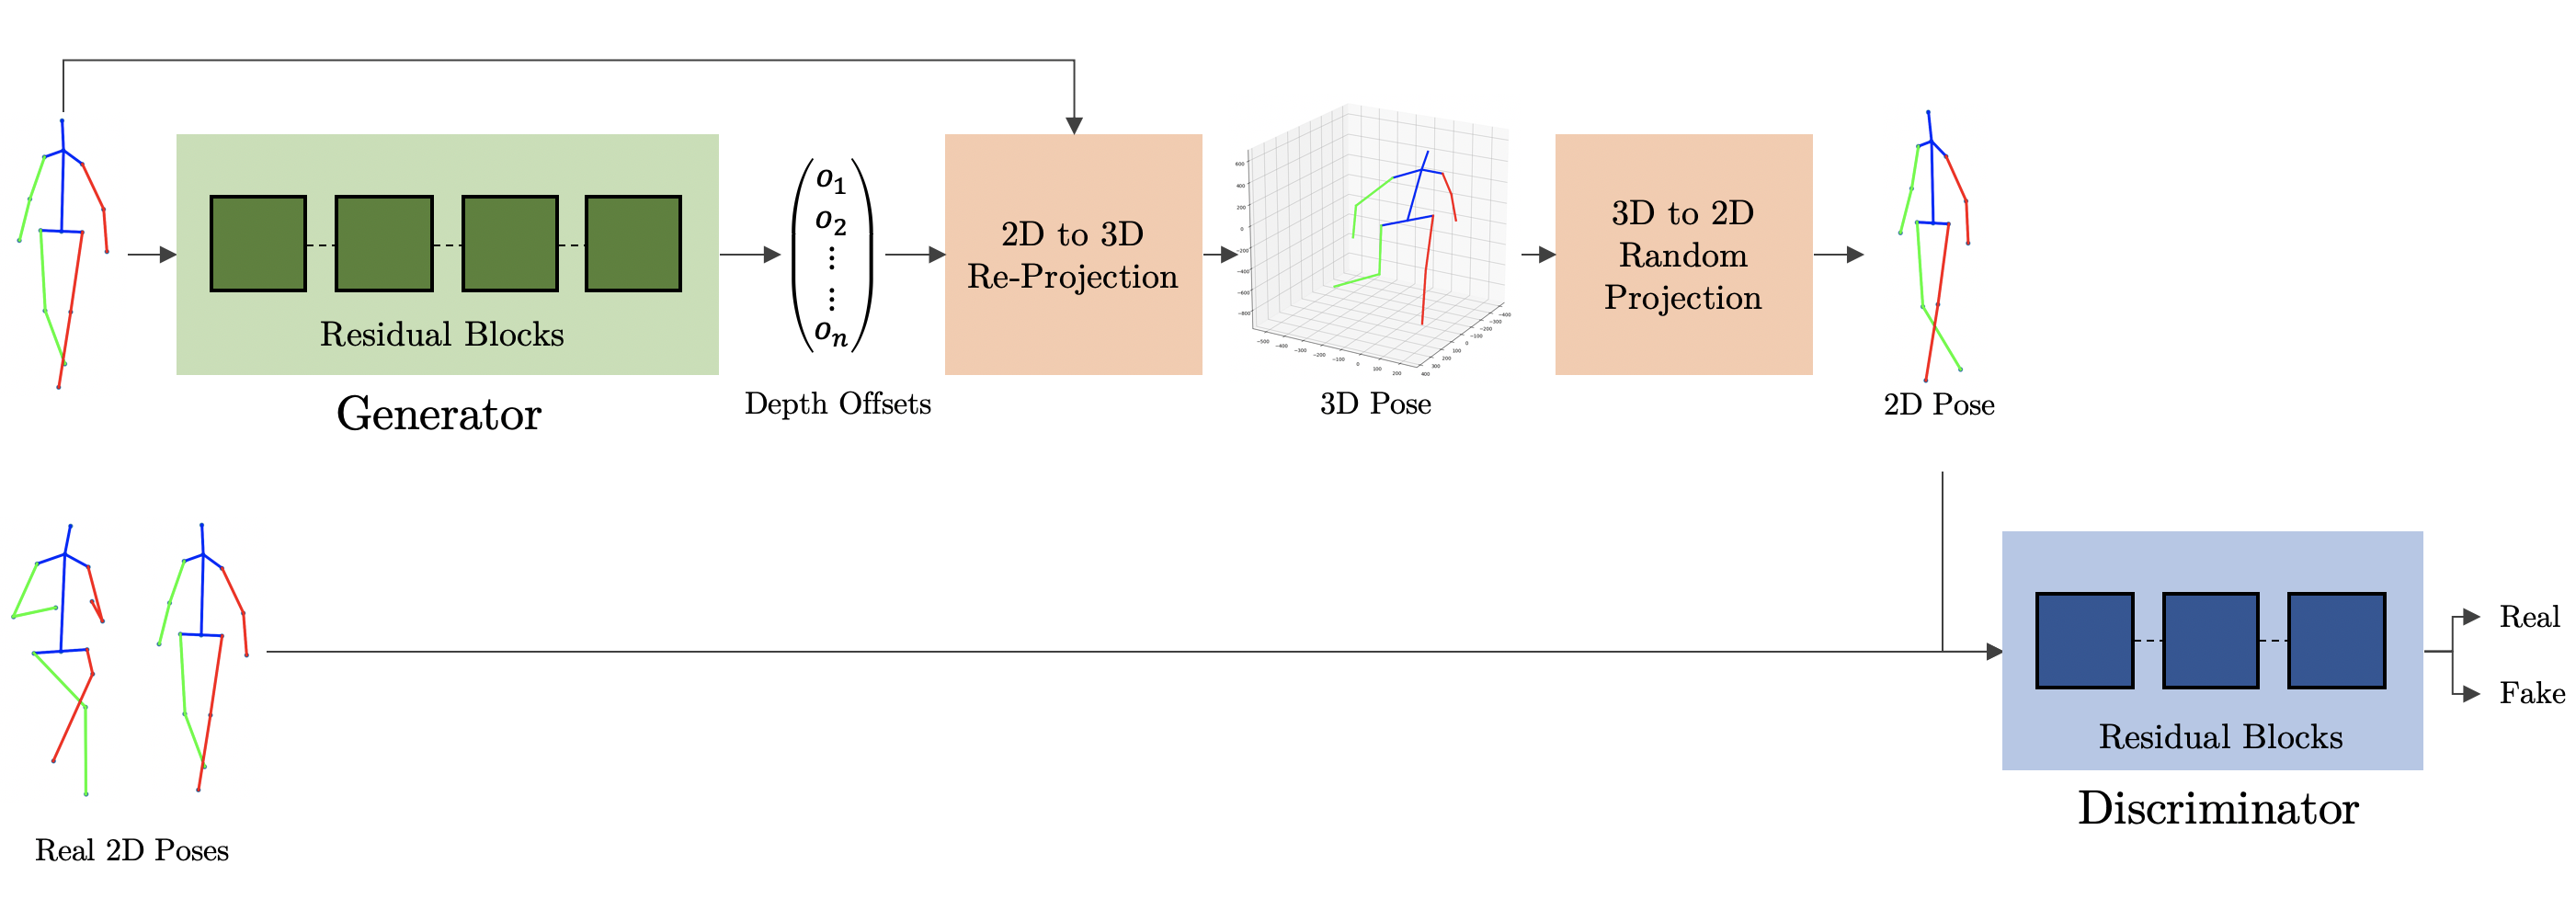
\includegraphics[width=1.1\textwidth]{figures/system.png}
	}
	\caption{The core of this thesis: The 2D to 3D pose GAN proposed by \citet{drover18}.}
	\label{fig:system}
\end{figure}

In production the generation process would be over at this point but for training, 2D poses have to be sampled from the reprojected 3D pose.
The 3D poses are aligned with the origin and randomly rotated with azimuth angles between $0$ and $360$ and elevation between $0$ between $20$ degrees.
\Todo{When 2D poses are sampled, the extrinsic parameters of the synthetic camera model should match those of the real camera(s)}

The \textit{discriminator} $D$ is defined as a neural network that consumes real 2D poses from the distribution $P_{real}$ and fake 2D poses drawn from $P_{fake}$ and outputs a scalar value in $[0, 1]$.

The loss functions used for the generator and the discriminator are the following \cite{goodfellow17}:
\begin{align}
	\label{eq:generator-loss}
	loss_G &= -\mathbb{E}_{p\sim P_{fake}}(\log(D(p))) \\
	\label{eq:discriminator-loss}
	loss_D &= -\frac{1}{2}\mathbb{E}_{r\sim P_{real}}(\log(D(r))) - \frac{1}{2} \mathbb{E}_{p\sim P_{fake}}(\log(1 - D(p)))
\end{align}

\Todo[inline]{Figure of residual blocks}

Both generator and discriminator consist of several consecutive \textit{residual blocks}.
A residual block consists of two fully connected layers of size $1024$ each followed by RELU activation and a residual connection adding the input to the last layer's output.
\citet{drover18} suggest two additional Batch Normalization layers \cite{ioffe15}, one immediately after each fully connected layer.
\Todo{Mention correspondence with other authors and code.}
Practical tests have shown that when using those additional layers the training does not converge at all.
\unsure{Wording of "auf die Batch Norm wurde verzichtet"}
As competitive results could also be achieved with the reduced network design, Batch Normalization has been left out completely in this work.

The generator takes $n$ 2D joint locations (i.e. $2n$ scalar inputs) as input and feeds them to a fully connected layer of size 1024.
This is followed by four of the residual blocks described above and concluded by another fully connected layer of size 1024 mapping the output of the last residual block to a vector of size $n$ representing the depth offset of each joint.
The 2D input and the estimated depth offsets are then combined to a 3D pose as described above.
From each predicted 3D pose a random 2D projection is created that is used for training.

\Todo{Figure of whole model: One "exit" to production right after the re-projection, one for training that goes into the 2D pose sampling layer}

The discriminator's architecture is very similar to the generator's. 
It also accepts $n$ 2D joint locations as input which are fed into a fully connected layer of size 1024, followed by three residual blocks.
The output is then reduced by another fully connected layer to a vector of size 2.
When softmax is applied during the error calculation, the values will imply the probability of the input being real or generated.

Assumptions:
\begin{enumerate}[label=(\Alph*)]
	\item The camera is centered at the root joint.
	\item The distance between the camera and the pose is (approximately) constant. 
\end{enumerate}
\begin{itemize}
	\item[(1)] All 2d data can be scaled in a way that a norm limb is of length 0.1. 
	Problems with correct camera distance, see section \ref{sec:z-shift-error}. 
	Problem when camera is perpendicular to the norm limb.
	\item[(2)] All data was captured with the same camera distance.
\end{itemize}